\chapter{LPE structure}

\section{Introduction}
The techniques that are described in this document require a \txs{} model as input that is in \emph{restricted model form}.
This form is a model-level version of the \emph{linear process equation} (LPE) form to which many, but not all \txs{} processes can be transformed using the \texttt{lpe} command of \txs{}.

\section{Restricted model form} \label{sec:restrictedmodelform}

A \txs{} model
\begin{align*}
\texttt{ModelDef} \; [I_1, \cdots{}, I_m] \; [O_1, \cdots{}, O_n] \; b_\textit{inst}
\end{align*}

is said to be in \emph{restricted model form} if

\begin{itemize}
\item $I_1, \cdots{}, I_m$ are all single input channels;
\item $O_1, \cdots{}, O_n$ are all single output channels;
\item $b_\text{\textit{inst}}$ has the form
\begin{align*}
\texttt{ProcInst} \; P \; [C_1, \cdots{}, C_{m+n}] \; [v_I(p_1), \cdots{}, v_I(p_k)]
\end{align*}

such that
\begin{align*}
\{ I_1, \cdots{}, I_m \}, \{ O_1, \cdots{}, O_n \} \subseteq \{ C_1, \cdots{}, C_{m+n} \}
\end{align*}

and
\begin{align*}
\{ I_1, \cdots{}, I_m \} \cap \{ O_1, \cdots{}, O_n \} = \emptyset{}
\end{align*}

\item the \txs{} process that is identified by $P$ is
\begin{align*}
\texttt{ProcDef} \; [C_1, \cdots{}, C_{m+n}] \; [p_1 :: T_1, \cdots{}, p_k :: T_k] \; b_\textit{LPE}
\end{align*}
such that $\text{type}(v_I(p_i)) = T_i$ for all $i \in [1, \cdots{}, k]$; and
\item the \txs{} process that is identified by $P$ is in LPE form (see \ref{sec:lpeform}).
\end{itemize}

\section{LPE form} \label{sec:lpeform}

A \txs{} process
\begin{align*}
\texttt{ProcDef} \; [C_1, \cdots{}, C_n] \; [p_1 :: T_1, \cdots{}, p_k :: T_k] \; b_\textit{LPE}
\end{align*}

that is identified by $P$ is said to be in \emph{LPE form} if $b_\textit{LPE}$ follows the grammar of $\textit{LPEBody}$ below:
\begin{align*}
\textit{LPEBody} &::= \textit{ChoiceSummand} \;|\; \textit{ActionSummand} \\
\textit{ChoiceSummand} &::= \texttt{Choice} \; [ \textit{LPEBody} ] \\
\textit{ActionSummand} &::= \texttt{ActionPref} \; \textit{ActOffer} \; \textit{ProcInst} \\
\textit{ActOffer} &::= \texttt{ActOffer} \; \textit{ActChan} \; [\texttt{Quest} \; x_1, \cdots{}, \texttt{Quest} \; x_m] \; \textit{VExpr} \\
\textit{ActChan} &::= [\;] \;|\; [C_1 \;| \cdots{} |\; C_n \;|\; \texttt{ISTEP} \;|\; \texttt{CISTEP}] \\
\textit{ProcInst} &::= P \; [C_1, \cdots{}, C_n] \; [\!\textit{VExpr}, \cdots{}, \textit{VExpr} ]
\end{align*}

Note that each of $x_1, \cdots{}, x_m$ can occur at most once in the list of communication variables of a summand!

\section{Data structure}

The implementation stores a \txs{} model that is in restricted model form in a dedicated data structure before any of the techniques that are described in this document are applied.
An overview of this data structure can be found in Figure~\ref{fig:lpedatastructure}.

\begin{figure}[!ht]
\begin{center}
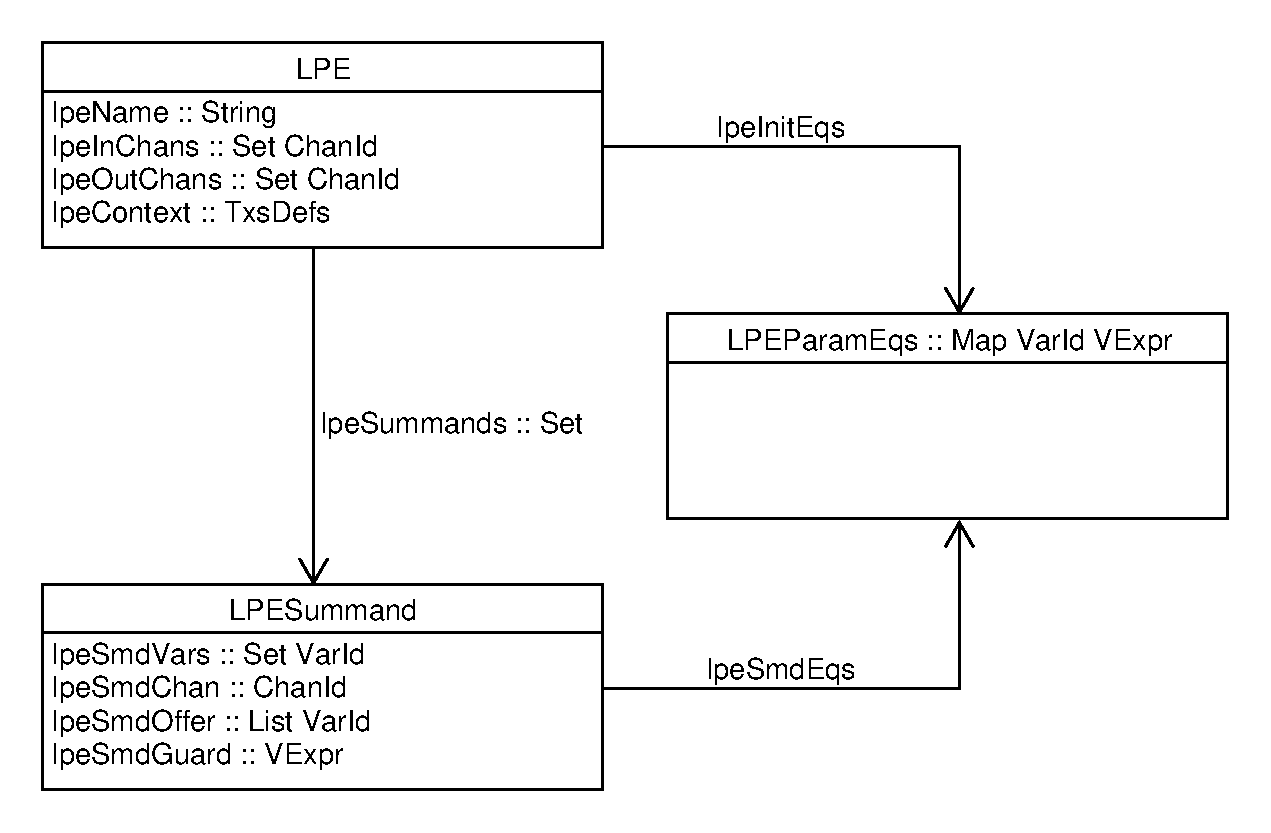
\includegraphics[width=0.7\linewidth]{images/lpe-types}
\caption{LPE data structure.}
\label{fig:lpedatastructure}
\end{center}
\end{figure}

The main data type is \texttt{LPE}, which is not a completely accurate name since it contains more information than only the linearized \txs{} process $P$, namely

\begin{itemize}
\item \texttt{lpeContext}, which is a library of \txs{} type and function definitions;
\item \texttt{lpeInChans}, which contains all channel parameters of $P$ that are input channels;
\item \texttt{lpeOutChans}, which contains all channel parameters of $P$ that are output channels; and
\item \texttt{lpeInitEqs}, which maps the data parameters of $P$ to their initial values.
\end{itemize}

The tree structure of summands that was allowed by the grammar of LPEs (see \ref{sec:lpeform}) has been flattened in the new data structure, resulting in a set of \texttt{LPESummand} objects that is part of the \texttt{LPE} data type.
These objects correspond with the \textit{ActionSummand} rule in the grammar.

One of the parts of the \texttt{LPESummand} data type is \texttt{lpeSmdVars}, which contains all variables that the summand uses besides LPE parameters.
These variables can be used in the channel offer, \texttt{lpeSmdOffer}, as communication variables (in a specific order); in the guard of the summand, \texttt{lpeSmdGuard}, an expression of sort \texttt{Bool}; and in the expressions that define the value of LPE parameters after the application of the summand, which are values in the \texttt{lpeSmdEqs} map.

\section{Example TODO}

The following code snippet gives a valid example of an LPE:

\begin{lstlisting}
//Process definition:
PROCDEF example[A :: Int, B](state, curr, prev :: Int)
  = A ? i [[state==0]] >-> example[A, B](2, i, prev)
  + A ? i [[state==1 && i!=prev]] >-> example[A, B](2, i, prev)
  + A ? i [[state==2 && i==curr]] >-> example[A, B](1, curr, curr)
  + B >-> STOP
  ;

//Initialization:
example[A, B](0, 0, 0);
\end{lstlisting}

The process only accepts input sequences in which every number is repeated exactly once.
The process terminates non-deterministically.
